\documentclass[conference]{IEEEtran}
\usepackage[T1]{fontenc}
\usepackage{cite}
\usepackage{amsmath,amssymb,amsfonts,amsthm}
\usepackage{algorithm}
\usepackage{algpseudocode}
\usepackage{booktabs}
\usepackage{graphicx}
\usepackage{xcolor}
\usepackage{listings}
\usepackage{tikz}
\usepackage{url}
\usepackage[hidelinks]{hyperref}
\graphicspath{{figures/}}

% ----------------------------------------------------------------- theorems
\newtheorem{theorem}{Theorem}
\newtheorem{lemma}{Lemma}
\newtheorem{corollary}{Corollary}
\theoremstyle{definition}
\newtheorem{definition}{Definition}
\theoremstyle{remark}
\newtheorem{remark}{Remark}

% --------------------------------------------------------------- notation
\newcommand{\TSM}{\textsc{Test-Suite-Min}}
\newcommand{\VC}{\textsc{Vertex-Cover}}
\newcommand{\SC}{\textsc{Set-Cover}}

% --------------------------------------------------------- code listings
\lstdefinestyle{code}{
  basicstyle=\ttfamily\scriptsize,
  numbers=left,
  numberstyle=\tiny\color{gray},
  numbersep=4pt,
  breaklines=true,
  breakatwhitespace=false,
  breakindent=1.5em,
  postbreak=\mbox{\textcolor{gray}{$\hookrightarrow$}\space},
  columns=fullflexible,
  keepspaces=true,
  showstringspaces=false,
  tabsize=4,
  frame=lines,
  xleftmargin=12pt,
  framexleftmargin=12pt,
  keywordstyle=\color{blue!60!black}\bfseries,
  commentstyle=\color{green!40!black}\itshape,
  stringstyle=\color{red!50!black}
}
\lstset{style=code}

\title{NP-Completeness in Practice:\\Regression Test-Suite Minimization}
\author{\IEEEauthorblockN{Avantika Holla Sathyanarayana}
\IEEEauthorblockA{Department of Computer and Information Science\\
University of Florida\\
Email: avantika.sathyan@ufl.edu}}

\begin{document}
\maketitle

\begin{abstract}
This report studies a problem shown to be NP-complete. It comes from
software engineering: a team wants the smallest subset of a regression test
suite that still checks every requirement. We model it as a set-covering
problem, prove its decision version NP-complete by a polynomial reduction
from \VC{}, and give a greedy algorithm that runs in $O(km + N + n)$ time and
returns at most $H(d) \le \ln d + 1$ times the optimal number of tests. A Java
implementation and reproducible benchmarks accompany it. The measured running
times are analyzed separately from the theoretical worst-case bounds; for the
greedy algorithm they match the fitted model with $R^2 = 0.992$, and on 630
small instances greedy is optimal 61\% of the time and never worse than
1.43 times the optimum.
\end{abstract}

\begin{IEEEkeywords}
NP-completeness, vertex cover, set cover, greedy algorithms,
regression testing, test-suite minimization
\end{IEEEkeywords}

\section{Introduction}
This report solves a practical problem with an algorithmic tool, following
the problem-to-algorithm structure: the real-world setting, its abstraction,
the reduction and proof, the algorithm, its complexity, an interpretation in
the application domain, a worked example, and experiments.

Section~\ref{sec:p2} presents regression test-suite minimization. As a
system evolves, its regression test suite keeps growing, and rerunning all of
it after every change becomes slow. Choosing the fewest tests that still check
every requirement is known in the software-engineering literature as
\emph{test-suite minimization}~\cite{harrold1993,yoo2012}. We show that this
problem is NP-complete, so no polynomial-time algorithm is expected to solve it
exactly, and we give and evaluate a greedy algorithm that solves it well in
practice.

The experiments characterize measured execution on synthetic inputs without
treating random-input behavior as a proof of the worst-case bounds. The
appendices contain the complete Java implementation and a disclosure of
AI-assisted development.

\section{Problem 2: NP-Completeness---Regression Test-Suite Minimization}
\label{sec:p2}

\subsection{Introduction}
\label{sec:p2-intro}
Software teams keep a \emph{regression test suite}: a collection of automated
tests that is rerun after every change to make sure that existing behavior
still works. Each test checks some of the system's \emph{testing
requirements}, such as functional requirements, statements or branches of the
code, or data-flow relationships~\cite{harrold1993}. As the software evolves,
new tests are added for new features and bug fixes, but old ones are rarely
removed. Many tests end up redundant, because other tests already check
everything they check, and running the whole suite after every commit wastes
time and computing resources.

\emph{Test-suite minimization} asks for the smallest subset of the suite that
still checks every requirement that the full suite checks. It is one of the
three main branches of regression-testing research, alongside test selection
and test prioritization~\cite{yoo2012}. Harrold, Gupta and Soffa introduced a
widely used heuristic for it~\cite{harrold1993}, and the problem is commonly
noted to be NP-complete~\cite{yoo2012}. In this section we prove
that claim from first principles and give a greedy algorithm.

\subsection{Problem Setting and Abstraction}
Number the requirements $1,\dots,n$ and the tests $1,\dots,m$. Test $i$ is
described only by the set of requirements it checks.

\begin{definition}[\TSM{}]
An instance consists of a finite universe $U = \{1,\dots,n\}$ of requirements
and a family $\mathcal{S} = (S_1,\dots,S_m)$ of subsets $S_i \subseteq U$,
where $S_i$ is the set of requirements checked by test $i$. A set of tests
$T \subseteq \{1,\dots,m\}$ is a \emph{covering suite} if
$\bigcup_{i\in T} S_i = U$.
\begin{itemize}
  \item \emph{Optimization version:} find a covering suite of minimum size $|T|$.
  \item \emph{Decision version} \TSM{}: given also an integer $k$, decide
        whether a covering suite with $|T| \le k$ exists.
\end{itemize}
\end{definition}

We assume without loss of generality that every requirement is checked by at
least one test (the instance is \emph{feasible}); a requirement that no test
checks can be detected in linear time and reported. We write
$N = \sum_{i=1}^{m} |S_i|$ for the total size of the input, and
$d = \max_i |S_i|$ for the largest number of requirements a single test checks.

This abstraction is exactly the input used by practical minimization tools,
which only need the association between each requirement and the tests that
satisfy it~\cite{harrold1993}. It is also a bipartite graph between tests and
requirements, with an edge whenever a test checks a requirement; $N$ is its
number of edges.

\subsection{Reduction from Vertex Cover}
To show that \TSM{} is NP-complete we prove two things: that it is NP-hard,
by reducing a known NP-complete problem to it, and that it is in NP. We
reduce from \VC{}, one of Karp's original NP-complete
problems~\cite{karp1972}.

\begin{definition}[\VC{}]
A \emph{vertex cover} of an undirected graph $G=(V,E)$ is a set of vertices
$C \subseteq V$ that contains at least one endpoint of every edge. Given $G$
and an integer $k$, \VC{} asks whether $G$ has a vertex cover with
$|C| \le k$.
\end{definition}

\subsubsection{Construction}
Let $(G, k)$ be an instance of \VC{} with vertices $V = \{v_1,\dots,v_p\}$ and
edges $E = \{e_1,\dots,e_q\}$. We build an instance $f(G,k)$ of \TSM{}:
\begin{itemize}
  \item one requirement $j$ for every edge $e_j$, so $U = \{1,\dots,q\}$;
  \item one test $i$ for every vertex $v_i$, which checks exactly the
        requirements of the edges incident to $v_i$:
        $S_i = \{\, j : v_i \in e_j \,\}$;
  \item the same budget $k$.
\end{itemize}
In software terms, think of each edge as a requirement that exactly two tests
check, namely the tests of its two endpoints.
The instance has $n = q$ requirements, $m = p$ tests and total size
$N = \sum_i |S_i| = \sum_i \deg(v_i) = 2q$. It is built with one pass over the
edge list, in $O(p + q)$ time, so the reduction is polynomial.
Fig.~\ref{fig:reduction} shows an example; our implementation is
\texttt{VertexCoverReduction} in Appendix~\ref{app:code}.

\begin{figure}[t]
\centering
\begin{minipage}{0.42\columnwidth}
\centering
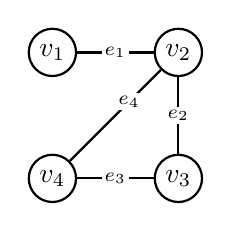
\begin{tikzpicture}[
    vertex/.style={circle, draw, thick, minimum size=6mm, inner sep=0pt},
    lbl/.style={font=\scriptsize, fill=white, inner sep=1pt}]
  \node[vertex] (a) at (0,1.6) {$v_1$};
  \node[vertex] (b) at (1.6,1.6) {$v_2$};
  \node[vertex] (c) at (1.6,0) {$v_3$};
  \node[vertex] (d) at (0,0) {$v_4$};
  \draw[thick] (a) -- node[lbl] {$e_1$} (b);
  \draw[thick] (b) -- node[lbl] {$e_2$} (c);
  \draw[thick] (c) -- node[lbl] {$e_3$} (d);
  \draw[thick] (b) -- node[lbl, pos=0.35] {$e_4$} (d);
\end{tikzpicture}
\end{minipage}%
\hfill
\begin{minipage}{0.55\columnwidth}
\centering\small
\begin{tabular}{@{}cl@{}}
\toprule
Test & Requirements checked \\
\midrule
$1$ & $S_1 = \{1\}$ \\
$2$ & $S_2 = \{1, 2, 4\}$ \\
$3$ & $S_3 = \{2, 3\}$ \\
$4$ & $S_4 = \{3, 4\}$ \\
\bottomrule
\end{tabular}
\end{minipage}
\caption{The reduction on a small graph. Each edge $e_j$ becomes requirement
$j$, and each vertex $v_i$ becomes test $i$, which checks the requirements of
its incident edges. The vertex cover $\{v_2, v_3\}$ corresponds to the covering
suite $\{2, 3\}$; both have the minimum size 2.}
\label{fig:reduction}
\end{figure}

\subsection{Proof of Correctness}
\begin{lemma}\label{lem:subset}
A set of vertices $C$ is a vertex cover of $G$ if and only if the
corresponding tests $T_C = \{\, i : v_i \in C \,\}$ check every requirement.
\end{lemma}
\begin{proof}
By the construction, test $i$ checks requirement $j$ exactly when vertex
$v_i$ is an endpoint of edge $e_j$. So requirement $j$ is checked by a test
in $T_C$ exactly when edge $e_j$ has an endpoint in $C$. This holds for every
$j$ at once, so all requirements are checked if and only if all edges are
covered.
\end{proof}

\begin{theorem}\label{thm:reduction}
$G$ has a vertex cover of size at most $k$ if and only if $f(G,k)$ has a
covering suite of size at most $k$. Hence $\VC{} \le_p \TSM{}$.
\end{theorem}
\begin{proof}
Each test corresponds to exactly one vertex, so a set of $k$ tests is the
same as a set of $k$ vertices. By Lemma~\ref{lem:subset}, one is a covering
suite exactly when the other is a vertex cover. The construction takes
polynomial time, so this is a polynomial-time reduction.
\end{proof}

It remains to show that a proposed answer can be checked quickly.

\begin{lemma}\label{lem:np}
\TSM{} is in NP.
\end{lemma}
\begin{proof}
Given a proposed list of tests $T$, we can check in polynomial time that
$|T| \le k$ and that every requirement is checked by some test in $T$: go
through the tests in $T$, mark the requirements they check, and see whether
all $n$ are marked. This takes $O(m + n + N)$ time
(\texttt{CoverageVerifier} in Appendix~\ref{app:code}).
\end{proof}

\begin{corollary}\label{cor:npc}
\TSM{} is NP-complete, and finding a smallest covering suite is NP-hard.
\end{corollary}
\begin{proof}
\VC{} is NP-complete~\cite{karp1972}, so Theorem~\ref{thm:reduction} makes
\TSM{} NP-hard, and Lemma~\ref{lem:np} puts it in NP. A fast algorithm for
the smallest suite would also answer the decision question (compare its size
with $k$), so that problem is NP-hard too.
\end{proof}

The reduction produces instances in which every requirement is checked by
exactly two tests, so the problem stays NP-hard even in that restricted case.

\begin{remark}[Reduction in the other direction]
The assignment asks for a reduction between the abstract problem and a known
NP-complete problem. Note the direction: Theorem~\ref{thm:reduction}
(known problem $\le_p$ our problem) is what proves hardness. The opposite
direction also holds trivially: an instance $(U,\mathcal{S},k)$ of \TSM{} is
literally an instance of \SC{}~\cite{karp1972}, with the same answer, so
$\TSM{} \le_p \SC{}$ by the identity map. Since \SC{} is in NP, this gives a
second proof of Lemma~\ref{lem:np}, and shows the two problems are
polynomially equivalent. On its own, however, a reduction from our problem to
a hard problem would not prove that our problem is hard.
\end{remark}

\subsection{Greedy Algorithm}
Because an exact polynomial-time algorithm is unlikely, we use the greedy rule
that the regression-testing literature also starts from~\cite{yoo2012}:
\emph{repeatedly run the test that checks the most requirements not yet
checked}, until every requirement is checked. Algorithm~\ref{alg:greedy}
implements this rule efficiently. It keeps, for each test $i$, a counter
$g[i]$ (the \emph{gain}) equal to the number of still-unchecked requirements in
$S_i$, and an inverted index $\mathit{byReq}[r]$ listing the tests that check
requirement $r$. When a requirement becomes checked, only the tests that
contain it lose gain, so the counters can be kept up to date cheaply.

\begin{algorithm}[t]
\caption{\textsc{GreedyMinimize}$(U, S_1,\dots,S_m)$}
\label{alg:greedy}
\begin{algorithmic}[1]
\For{$r \gets 1$ \textbf{to} $n$} $\mathit{byReq}[r] \gets$ empty list
\EndFor
\For{$i \gets 1$ \textbf{to} $m$}
  \State $g[i] \gets |S_i|$
  \For{each $r \in S_i$} append $i$ to $\mathit{byReq}[r]$
  \EndFor
\EndFor
\State $\mathit{checked}[1..n] \gets \textbf{false}$;\; $\mathit{left} \gets n$;\; $T \gets \emptyset$
\While{$\mathit{left} > 0$}
  \State $b \gets \arg\max_{i} g[i]$ \Comment{ties: smallest index}
  \If{$g[b] = 0$} \Return ``infeasible'' \EndIf
  \State $T \gets T \cup \{b\}$
  \For{each $r \in S_b$ with $\neg\mathit{checked}[r]$}
    \State $\mathit{checked}[r] \gets \textbf{true}$;\; $\mathit{left} \gets \mathit{left} - 1$
    \For{each $i \in \mathit{byReq}[r]$} $g[i] \gets g[i] - 1$
    \EndFor
  \EndFor
\EndWhile
\State \Return $T$
\end{algorithmic}
\end{algorithm}

\paragraph*{Correctness}
The algorithm maintains the invariant
$g[i] = |\{\, r \in S_i : \neg\mathit{checked}[r] \,\}|$ for every test $i$.
It holds after initialization, when nothing is checked. Each requirement $r$
is marked checked exactly once, and at that moment every test containing $r$,
and only those, has its gain decreased by one, which restores the invariant.

\begin{lemma}\label{lem:greedy-valid}
If every requirement is checked by some test, Algorithm~\ref{alg:greedy}
returns a covering suite after at most $\min(m, n)$ iterations.
\end{lemma}
\begin{proof}
While some requirement is unchecked, a test containing it has gain at least
1, so the chosen test checks at least one new requirement. Hence each
iteration checks a new requirement (at most $n$ iterations), and a chosen test
has gain 0 afterwards, so it is never chosen twice (at most $m$ iterations).
The loop stops only when every requirement is checked. If some requirement is
in no test, all gains eventually reach 0 and the algorithm reports
``infeasible''.
\end{proof}

\paragraph*{Quality guarantee}
Greedy is not always optimal (an example follows in
Section~\ref{sec:p2-example}), but it is never far off.

\begin{theorem}[\cite{chvatal1979}]\label{thm:approx}
Greedy returns at most $H(d)\cdot\mathrm{OPT}$ tests, where $\mathrm{OPT}$ is
the size of a smallest covering suite and
$H(d) = 1 + \tfrac12 + \dots + \tfrac1d \le \ln d + 1$.
\end{theorem}
\begin{proof}[Proof sketch]
Each time greedy picks a test that checks $c$ new requirements, give each of
them a cost of $1/c$. Every pick hands out a total cost of 1, so the total
cost equals the number of tests greedy picks. Now take any test $S$ of an
optimal suite. When the $t$-th last of its requirements is checked, $S$
itself would still check at least $t$ new ones, so greedy's pick checks at
least $t$ and that requirement costs at most $1/t$. The requirements of $S$
therefore cost at most $1 + \tfrac12 + \dots + \tfrac1d = H(d)$ in total.
Every requirement is in some test of the optimal suite, so the total cost,
and hence greedy's number of tests, is at most $H(d)\cdot\mathrm{OPT}$.
\end{proof}

\subsection{Running Time and Space Analysis}
Let $k = |T|$ be the number of tests greedy selects; by
Lemma~\ref{lem:greedy-valid}, $k \le \min(m,n)$.
\begin{itemize}
  \item Building the gains and the inverted index (lines 1--6) touches every
        pair $(i, r)$ with $r \in S_i$ once: $O(m + n + N)$.
  \item Each iteration finds $\arg\max_i g[i]$ by scanning all $m$ counters:
        $O(km)$ over the whole run.
  \item Each requirement is marked checked once, and at that moment the
        algorithm walks its list $\mathit{byReq}[r]$. The lists have total
        length $N$, so all the gain updates together cost $O(N)$. Scanning
        $S_b$ for each chosen test is also $O(N)$ in total, since each test is
        chosen at most once.
\end{itemize}
Hence
\[
T_{\text{greedy}}(m,n,N) = O(km + N + n).
\]
In the worst case $k = \min(m,n)$ and $N \le mn$, giving $O(mn)$, which is
linear in the size of the test-by-requirement matrix. Memory is $O(m + n + N)$.
A priority queue would replace the $O(km)$ scan with $O(N \log m)$ heap
updates; we use the scan because it is simpler and, as the experiments show, it
is very fast in practice.

\subsection{Explanation in the Language of the Problem Domain}
\label{sec:p2-domain}
Start with nothing selected. Look at every test and count how many
requirements it would check that no selected test checks yet; run the test
with the highest count, and repeat until every requirement is checked. A test
whose requirements are all already checked by selected tests has count zero
and is never selected, which is exactly how redundant tests are dropped.

Minimizing only preserves the requirements that are modeled. A removed test
may still have been able to reveal faults that the remaining tests miss, and
studies have found that fault-detection ability can drop noticeably in
practice~\cite{rothermel1998}. A team can limit this risk by
minimizing with fine-grained requirements, or by keeping the full suite for
nightly runs and using the minimized one after each commit.

\subsection{Worked Example and Execution Trace}
\label{sec:p2-example}
Consider a web shop with six requirements: login ($r_1$), logout ($r_2$),
password reset ($r_3$), checkout ($r_4$), refund ($r_5$) and invoice ($r_6$).
The suite has three tests: an \emph{authentication} test
$S_1=\{r_1,r_2,r_3\}$, a \emph{payments} test $S_2=\{r_4,r_5,r_6\}$, and a
long end-to-end \emph{smoke} test $S_3=\{r_2,r_3,r_5,r_6\}$.

Initially the gains are $(g_1,g_2,g_3)=(3,3,4)$, so greedy selects the smoke
test, which checks $r_2,r_3,r_5,r_6$. Each of these requirements lowers the
gain of the other test that contains it, leaving $(1,1,0)$. Greedy then
selects the authentication test for $r_1$ (a tie, broken by the smaller
index), and finally the payments test for $r_4$. It returns three tests,
$\{S_3,S_1,S_2\}$, while the optimum is two, $\{S_1,S_2\}$. The ratio $3/2$
is within the guarantee of Theorem~\ref{thm:approx}, since
$H(4)\approx 2.08$ here.

\subsection{Implementation and Verification}
We implemented the abstraction, the verifier, the reduction, the greedy
algorithm and an exact branch-and-bound solver in Java
(Appendix~\ref{app:code}). Twenty-six unit tests pass. One checks
Lemma~\ref{lem:subset} exhaustively: on 200 random graphs with up to 10
vertices, for \emph{every} subset of vertices, the subset is a vertex cover
exactly when the corresponding tests form a covering suite. Another compares
the exact solver against brute force on 200 random instances and checks that
greedy's output is always a valid cover within $H(d)\cdot\mathrm{OPT}$. These
are implementation checks rather than a substitute for the proofs.

\subsection{Experimental Evaluation}
\label{sec:p2-experiments}
\subsubsection{Experimental Setup}
Running time was measured on random instances with $m = n$ from 500 to
12{,}000, in two families. In the \emph{sparse} family each test checks about
20 requirements on average, so $N \approx 20m$. In the \emph{dense} family
each test checks each requirement with probability $p = 0.05$, so
$N \approx 0.05\,mn$. Every requirement is guaranteed to be checked by some
test. For each instance we ran 5 warm-up runs and report the median of 21
timed runs. All instances are generated from fixed seeds and are reproducible
exactly.

\subsubsection{Running Time}
The two families exercise different terms of the bound. In the sparse family
greedy needs many tests ($k \approx 0.087m$), so the $km$ scan dominates; in
the dense family $k$ grows slowly (from 38 to 74) and the $N$ term dominates.
Because the two terms do different kinds of work (a sequential scan versus
scattered counter updates), we fitted one constant per term,
\[
T(m,n,N) \approx a\cdot km + b\cdot (N + n),
\]
by non-negative least squares over both families, obtaining
$a = 0.186$~ns, $b = 3.07$~ns and $R^2 = 0.992$.

\begin{figure}[t]
\centering
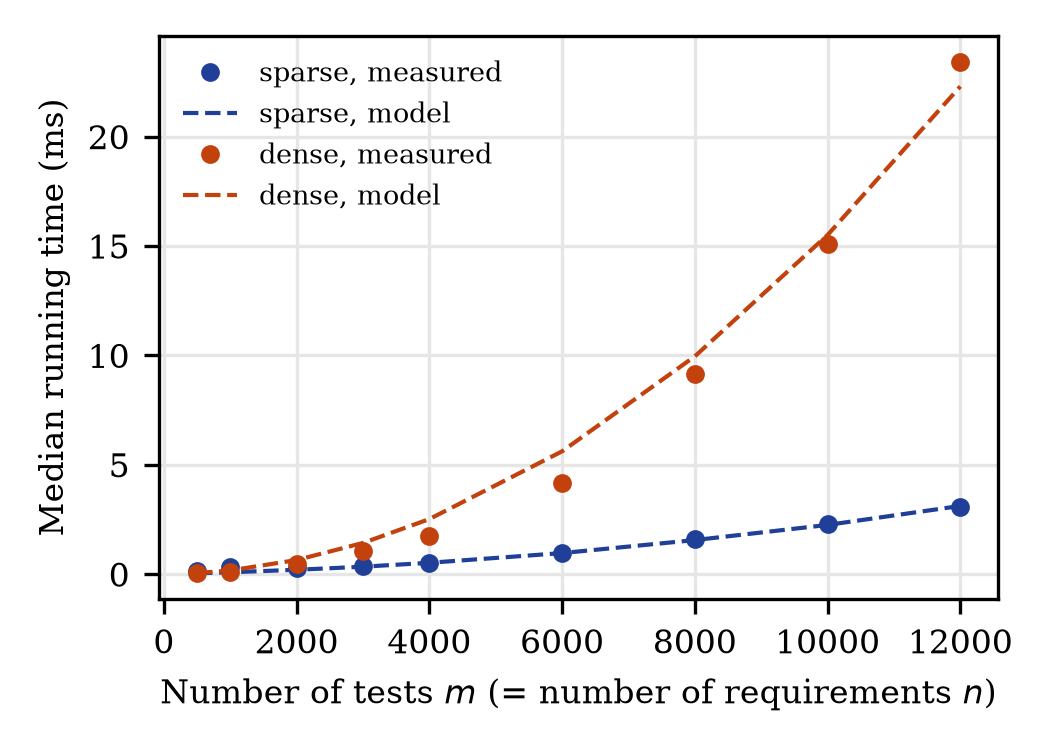
\includegraphics[width=\columnwidth]{figures/runtime.png}
\caption{Median running time of greedy for both instance families (markers)
and the fitted model $a\cdot km + b\cdot(N+n)$ (dashed).}
\label{fig:runtime}
\end{figure}

\begin{figure}[t]
\centering
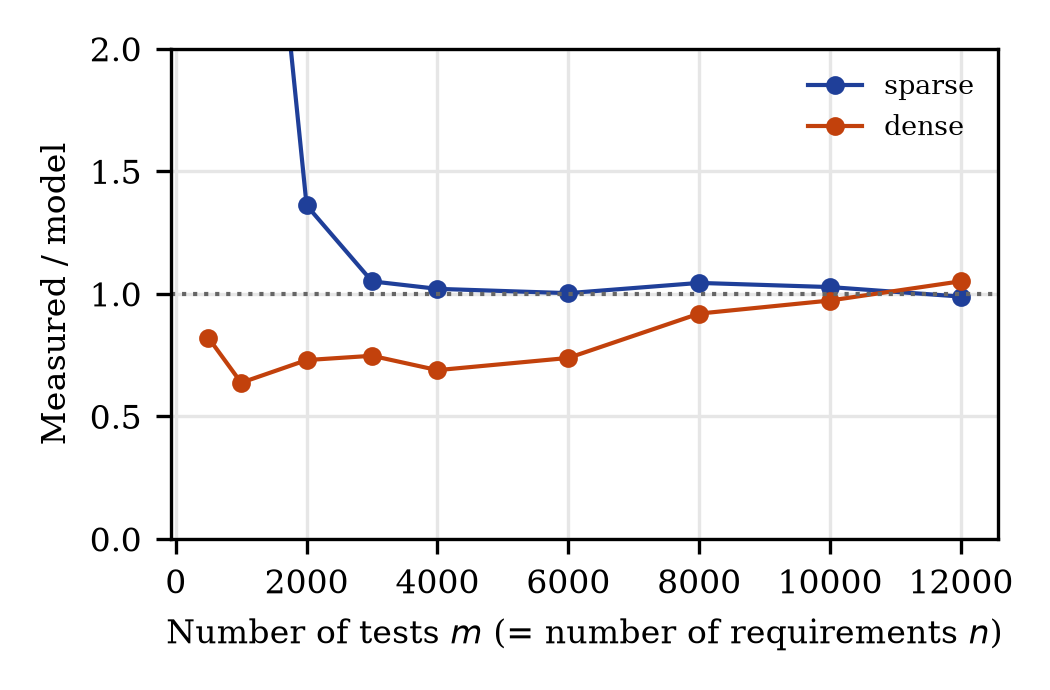
\includegraphics[width=\columnwidth]{figures/ratio.png}
\caption{Ratio of measured time to the fitted model. A flat line at 1 means
the time grows exactly as the analysis predicts. The sparse ratio for the two
smallest sizes (4.4 and 4.0) is cut off.}
\label{fig:ratio}
\end{figure}

\begin{table}[t]
\centering
\caption{Measured greedy running times (median of 21 runs).}
\label{tab:runtime}
\small
\setlength{\tabcolsep}{4pt}
\begin{tabular}{@{}r rrr rrr@{}}
\toprule
 & \multicolumn{3}{c}{Sparse} & \multicolumn{3}{c}{Dense ($p=0.05$)} \\
\cmidrule(lr){2-4}\cmidrule(l){5-7}
$m = n$ & $N$ & $k$ & ms & $N$ & $k$ & ms \\
\midrule
500    &   9{,}904 &    45 & 0.158 &    12{,}454 & 38 &  0.036 \\
1{,}000  &  19{,}810 &    86 & 0.320 &    49{,}872 & 43 &  0.105 \\
2{,}000  &  40{,}140 &   175 & 0.265 &   200{,}017 & 51 &  0.466 \\
3{,}000  &  59{,}982 &   253 & 0.352 &   449{,}830 & 54 &  1.060 \\
4{,}000  &  79{,}890 &   343 & 0.523 &   800{,}248 & 57 &  1.728 \\
6{,}000  & 119{,}651 &   512 & 0.961 & 1{,}798{,}679 & 63 &  4.140 \\
8{,}000  & 159{,}877 &   695 & 1.620 & 3{,}201{,}885 & 67 &  9.145 \\
10{,}000 & 200{,}184 &   858 & 2.306 & 4{,}997{,}856 & 70 & 15.071 \\
12{,}000 & 239{,}702 & 1{,}046 & 3.076 & 7{,}197{,}823 & 74 & 23.426 \\
\bottomrule
\end{tabular}
\end{table}

Fig.~\ref{fig:runtime} and Table~\ref{tab:runtime} show the measurements, and
Fig.~\ref{fig:ratio} the ratio of measured to modeled time. For the sparse
family the ratio stays between 0.99 and 1.05 from $m = 3{,}000$ upward, so the
running time grows exactly as the analysis predicts. Below that size the runs
take a fraction of a millisecond, and fixed costs that the model ignores, such
as allocating the arrays and the resolution of the timer, dominate. For the
dense family the ratio stays between 0.64 and 0.82 up to $m = 6{,}000$ and
then rises to 1.05 as $N$ grows to $7.2\times 10^6$. A likely explanation is the memory
hierarchy: the gain updates jump around the counter array, and once the
inverted index no longer fits in the processor's cache each update costs more.
The number of operations still follows the analysis; only the cost per
operation changes, which a constant-cost model cannot capture.

\begin{figure}[t]
\centering
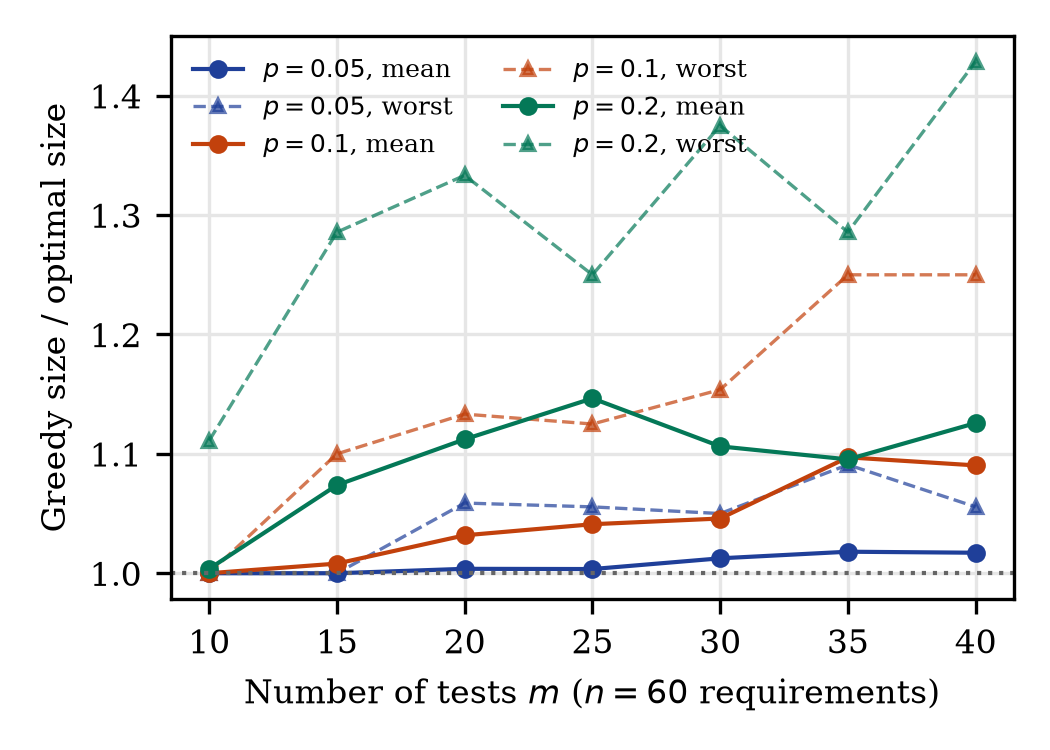
\includegraphics[width=\columnwidth]{figures/quality.png}
\caption{Greedy suite size divided by the optimal size on small random
instances ($n = 60$; 30 instances per point). The theoretical bound $H(d)$ is
between 2.28 and 3.82 for these instances, above the top of the plot.}
\label{fig:quality}
\end{figure}

\begin{table}[t]
\centering
\caption{Greedy versus optimal on 630 small random instances.}
\label{tab:quality}
\small
\begin{tabular}{@{}lrrr@{}}
\toprule
Density $p$ & Greedy optimal & Mean ratio & Worst ratio \\
\midrule
0.05 & 83.8\% & 1.008 & 1.091 \\
0.10 & 55.7\% & 1.045 & 1.250 \\
0.20 & 42.9\% & 1.095 & 1.429 \\
\midrule
All  & 60.8\% & 1.049 & 1.429 \\
\bottomrule
\end{tabular}
\end{table}

\subsubsection{Solution Quality}
To measure solution quality we compared greedy with the exact optimum, computed
by branch and bound, on 630 instances with $n = 60$ requirements,
$m \in \{10, 15, \dots, 40\}$ tests and densities $p \in \{0.05, 0.10, 0.20\}$
(30 instances per setting). Fig.~\ref{fig:quality} and
Table~\ref{tab:quality} summarize the results. Greedy found an optimal suite
in 61\% of the instances, used 4.9\% more tests than necessary on average, and
was never worse than 1.43 times the optimum, well inside the guarantee of
Theorem~\ref{thm:approx} ($H(d) \ge 2.28$ here). Greedy does worse when tests
overlap more (larger $p$) and when there are more tests to choose from, since
both create more opportunities for an early choice like the smoke test of
Section~\ref{sec:p2-example} to be misleading.

\subsubsection{Limitations and Validity}
The instances are random and synthetic, and each was timed in a single JVM
process. Real test suites have structured coverage, with groups of tests that
overlap heavily, so greedy's quality on them may differ from
Table~\ref{tab:quality}. The quality comparison is limited to small instances
because the exact solver takes exponential time. These measurements show how
the algorithm scales on the tested inputs; they do not prove the worst-case
bound, which comes from the analysis above.

\section{Conclusion}
Regression test-suite minimization is a set-covering problem in disguise. The
reduction from \VC{} shows that it is NP-complete even when every requirement is
checked by exactly two tests, so we do not expect an efficient exact algorithm.
The greedy rule of always running the test that checks the most unchecked
requirements runs in $O(km + N + n)$ time, which our experiments confirmed
($R^2 = 0.992$), and it is guaranteed to be within a factor $H(d)$ of optimal.
In practice it did much better than that guarantee: on 630 random instances it
was optimal 61\% of the time and never more than 1.43 times the optimum.
Natural extensions are tests with different running times (weighted set cover)
and keeping some redundancy so that minimization does not reduce the suite's
ability to find faults~\cite{rothermel1998}.

\begin{thebibliography}{00}

\bibitem{harrold1993} M.~J. Harrold, R.~Gupta, and M.~L. Soffa, ``A methodology
for controlling the size of a test suite,'' \emph{ACM Transactions on Software
Engineering and Methodology}, vol.~2, no.~3, pp.~270--285, Jul. 1993.

\bibitem{yoo2012} S.~Yoo and M.~Harman, ``Regression testing minimization,
selection and prioritization: A survey,'' \emph{Software Testing, Verification
and Reliability}, vol.~22, no.~2, pp.~67--120, 2012.

\bibitem{karp1972} R.~M. Karp, ``Reducibility among combinatorial problems,'' in
\emph{Complexity of Computer Computations}, R.~E. Miller and J.~W. Thatcher,
Eds. New York: Plenum Press, 1972, pp.~85--103.

\bibitem{chvatal1979} V.~Chv{\'a}tal, ``A greedy heuristic for the set-covering
problem,'' \emph{Mathematics of Operations Research}, vol.~4, no.~3,
pp.~233--235, 1979.

\bibitem{rothermel1998} G.~Rothermel, M.~J. Harrold, J.~Ostrin, and C.~Hong,
``An empirical study of the effects of minimization on the fault detection
capabilities of test suites,'' in \emph{Proc. Int. Conf. Software
Maintenance}. IEEE, 1998, pp.~34--43.

\end{thebibliography}

\appendices
\section{Implementation and Reproducibility}
\label{app:code}
\subsection{Problem 2: Regression Test-Suite Minimization}
The Problem 2 project (Maven, Java 17+) is organized in the package
\texttt{testmin}. The following subsections list its source files.

\subsection{Problem 2: Model}
\begin{lstlisting}[style=code,language=Java]
package testmin.model;

import java.util.Arrays;

/**
 * One regression test and the set of requirements it covers.
 */
public final class TestCase {

    private final int id;
    private final int[] covers;

    /**
     * @param id     test id; must equal this test's index in its {@link Instance}
     * @param covers requirement ids covered by this test (duplicates are removed)
     * @throws IllegalArgumentException if {@code id} or any requirement id is negative
     */
    public TestCase(int id, int[] covers) {
        if (id < 0) {
            throw new IllegalArgumentException("Test id must be non-negative: " + id);
        }
        int[] sorted = covers.clone();
        Arrays.sort(sorted);
        if (sorted.length > 0 && sorted[0] < 0) {
            throw new IllegalArgumentException("Requirement ids must be non-negative: " + sorted[0]);
        }
        this.id = id;
        this.covers = dedupSorted(sorted);
    }

    private static int[] dedupSorted(int[] sorted) {
        if (sorted.length == 0) {
            return sorted;
        }
        int unique = 1;
        for (int i = 1; i < sorted.length; i++) {
            if (sorted[i] != sorted[unique - 1]) {
                sorted[unique++] = sorted[i];
            }
        }
        return unique == sorted.length ? sorted : Arrays.copyOf(sorted, unique);
    }

    public int id() {
        return id;
    }

    /** Number of distinct requirements this test covers. */
    public int size() {
        return covers.length;
    }

    /** The {@code i}-th covered requirement id (ascending order). Allocation-free access for hot loops. */
    public int requirement(int i) {
        return covers[i];
    }

    /** Defensive copy of the covered requirement ids, in ascending order. */
    public int[] covers() {
        return covers.clone();
    }

    /** Largest requirement id covered, or -1 if this test covers nothing. */
    public int maxRequirement() {
        return covers.length == 0 ? -1 : covers[covers.length - 1];
    }

    @Override
    public boolean equals(Object o) {
        return o instanceof TestCase other && id == other.id && Arrays.equals(covers, other.covers);
    }

    @Override
    public int hashCode() {
        return 31 * Integer.hashCode(id) + Arrays.hashCode(covers);
    }

    @Override
    public String toString() {
        return "t" + id + Arrays.toString(covers);
    }
}
\end{lstlisting}

\begin{lstlisting}[style=code,language=Java]
package testmin.model;

import java.util.List;

/**
 * An instance of Test-Suite Minimization: a universe of requirements
 * {@code U = {0, ..., n-1}} and a list of tests, each covering a subset of U.
 */
public final class Instance {

    private final int numRequirements;
    private final List<TestCase> tests;
    private final long totalCoverageSize;

    /**
     * @throws IllegalArgumentException if ids are inconsistent or a test covers
     *                                  a requirement outside {@code [0, numRequirements)}
     */
    public Instance(int numRequirements, List<TestCase> tests) {
        if (numRequirements < 0) {
            throw new IllegalArgumentException("numRequirements must be non-negative: " + numRequirements);
        }
        List<TestCase> copy = List.copyOf(tests); // also rejects null elements
        long total = 0;
        for (int i = 0; i < copy.size(); i++) {
            TestCase t = copy.get(i);
            if (t.id() != i) {
                throw new IllegalArgumentException("Test at index " + i + " has id " + t.id());
            }
            if (t.maxRequirement() >= numRequirements) {
                throw new IllegalArgumentException(
                        "Test " + i + " covers requirement " + t.maxRequirement()
                                + " but only " + numRequirements + " exist");
            }
            total += t.size();
        }
        this.numRequirements = numRequirements;
        this.tests = copy;
        this.totalCoverageSize = total;
    }

    /** n = |U|. */
    public int numRequirements() {
        return numRequirements;
    }

    /** m = number of tests. */
    public int numTests() {
        return tests.size();
    }

    public TestCase test(int id) {
        return tests.get(id);
    }

    /** Unmodifiable view of all tests. */
    public List<TestCase> tests() {
        return tests;
    }

    /** N = sum of |S_i| over all tests: the input size that drives running time. */
    public long totalCoverageSize() {
        return totalCoverageSize;
    }

    /** True iff every requirement is covered by at least one test (i.e. some solution exists). */
    public boolean isFeasible() {
        boolean[] covered = new boolean[numRequirements];
        int remaining = numRequirements;
        for (TestCase t : tests) {
            for (int i = 0; i < t.size(); i++) {
                int r = t.requirement(i);
                if (!covered[r]) {
                    covered[r] = true;
                    remaining--;
                }
            }
        }
        return remaining == 0;
    }
}
\end{lstlisting}

\begin{lstlisting}[style=code,language=Java]
package testmin.model;

import java.util.List;

/**
 * A selection of tests, identified by test id, in the order they were chosen.
 */
public record Solution(List<Integer> selectedTestIds) {

    public Solution {
        selectedTestIds = List.copyOf(selectedTestIds);
    }

    /** Number of selected tests: the quantity being minimized. */
    public int size() {
        return selectedTestIds.size();
    }
}
\end{lstlisting}
\begin{lstlisting}[style=code,language=Java]
package testmin.model;

/** Thrown when some requirement is not covered by any test, so no solution exists. */
public class InfeasibleInstanceException extends RuntimeException {

    private static final long serialVersionUID = 1L;

    public InfeasibleInstanceException(String message) {
        super(message);
    }
}
\end{lstlisting}


\subsection{Problem 2: Algorithms}
\begin{lstlisting}[style=code,language=Java]
package testmin.algo;

import testmin.model.InfeasibleInstanceException;
import testmin.model.Instance;
import testmin.model.Solution;

/** Strategy for choosing a subset of tests that covers every requirement. */
public interface Minimizer {

    /**
     * Returns a set of tests covering every requirement of {@code instance}.
     *
     * @throws InfeasibleInstanceException if some requirement is covered by no test
     */
    Solution solve(Instance instance);

    /** Short human-readable name, used in benchmark output. */
    String name();
}
\end{lstlisting}

\begin{lstlisting}[style=code,language=Java]
package testmin.algo;

import testmin.model.Instance;
import testmin.model.TestCase;

/**
 * Inverted index: for each requirement r, the ids of the tests that cover r.
 */
final class CoverageIndex {

    private CoverageIndex() {
    }

    /** {@code result[r]} lists the ids of tests covering requirement r, in ascending order. */
    static int[][] build(Instance instance) {
        int n = instance.numRequirements();
        int[] counts = new int[n];
        for (TestCase t : instance.tests()) {
            for (int i = 0; i < t.size(); i++) {
                counts[t.requirement(i)]++;
            }
        }
        int[][] coveredBy = new int[n][];
        for (int r = 0; r < n; r++) {
            coveredBy[r] = new int[counts[r]];
        }
        int[] fill = new int[n];
        for (TestCase t : instance.tests()) {
            for (int i = 0; i < t.size(); i++) {
                int r = t.requirement(i);
                coveredBy[r][fill[r]++] = t.id();
            }
        }
        return coveredBy;
    }
}
\end{lstlisting}

\begin{lstlisting}[style=code,language=Java]
package testmin.algo;

import java.util.ArrayList;
import java.util.List;
import testmin.model.InfeasibleInstanceException;
import testmin.model.Instance;
import testmin.model.Solution;
import testmin.model.TestCase;

/**
 * Greedy test-suite minimization: repeatedly select the test that covers the
 * most still-uncovered requirements (ties broken by smallest id).
 */
public final class GreedyMinimizer implements Minimizer {

    @Override
    public Solution solve(Instance instance) {
        int m = instance.numTests();
        int n = instance.numRequirements();
        int[][] coveredBy = CoverageIndex.build(instance);

        // gain[t] = number of requirements covered by t that are not yet covered.
        int[] gain = new int[m];
        for (int t = 0; t < m; t++) {
            gain[t] = instance.test(t).size();
        }

        boolean[] covered = new boolean[n];
        int remaining = n;
        List<Integer> selected = new ArrayList<>();

        while (remaining > 0) {
            int best = argMax(gain);
            if (best < 0 || gain[best] == 0) {
                throw new InfeasibleInstanceException(
                        remaining + " requirement(s) are not covered by any test");
            }
            selected.add(best);

            TestCase chosen = instance.test(best);
            for (int i = 0; i < chosen.size(); i++) {
                int r = chosen.requirement(i);
                if (!covered[r]) {
                    covered[r] = true;
                    remaining--;
                    for (int t : coveredBy[r]) {
                        gain[t]--;
                    }
                }
            }
        }
        return new Solution(selected);
    }

    /** Index of the largest value (first one on ties), or -1 for an empty array. */
    private static int argMax(int[] values) {
        int best = -1;
        int bestValue = Integer.MIN_VALUE;
        for (int i = 0; i < values.length; i++) {
            if (values[i] > bestValue) {
                bestValue = values[i];
                best = i;
            }
        }
        return best;
    }

    @Override
    public String name() {
        return "greedy";
    }
}
\end{lstlisting}

\begin{lstlisting}[style=code,language=Java]
package testmin.algo;

import java.util.ArrayList;
import java.util.List;
import testmin.model.InfeasibleInstanceException;
import testmin.model.Instance;
import testmin.model.Solution;
import testmin.model.TestCase;

/**
 * Exact (optimal) test-suite minimization by branch and bound.
 */
public final class ExactMinimizer implements Minimizer {

    @Override
    public Solution solve(Instance instance) {
        if (!instance.isFeasible()) {
            throw new InfeasibleInstanceException("Some requirement is not covered by any test");
        }
        List<Integer> upperBound = new GreedyMinimizer().solve(instance).selectedTestIds();
        Search search = new Search(instance, upperBound);
        search.run(0);
        return new Solution(search.best);
    }

    @Override
    public String name() {
        return "exact";
    }

    /** Mutable state for one branch-and-bound run. */
    private static final class Search {
        private final Instance instance;
        private final int[][] coveredBy;
        private final int[] coverCount; // how many selected tests cover each requirement
        private final List<Integer> current = new ArrayList<>();
        private int uncovered;
        private List<Integer> best;

        Search(Instance instance, List<Integer> initialBest) {
            this.instance = instance;
            this.coveredBy = CoverageIndex.build(instance);
            this.coverCount = new int[instance.numRequirements()];
            this.uncovered = instance.numRequirements();
            this.best = new ArrayList<>(initialBest);
        }

        /** Invariant: every requirement below {@code firstCandidate} is covered. */
        void run(int firstCandidate) {
            if (uncovered == 0) {
                if (current.size() < best.size()) {
                    best = new ArrayList<>(current);
                }
                return;
            }
            // At least one more test is needed, so only continue if that could beat the best.
            if (current.size() + 1 >= best.size()) {
                return;
            }
            int r = firstCandidate;
            while (coverCount[r] > 0) {
                r++;
            }
            for (int t : coveredBy[r]) {
                add(t);
                current.add(t);
                run(r + 1);
                current.remove(current.size() - 1);
                remove(t);
            }
        }

        private void add(int testId) {
            TestCase t = instance.test(testId);
            for (int i = 0; i < t.size(); i++) {
                if (coverCount[t.requirement(i)]++ == 0) {
                    uncovered--;
                }
            }
        }

        private void remove(int testId) {
            TestCase t = instance.test(testId);
            for (int i = 0; i < t.size(); i++) {
                if (--coverCount[t.requirement(i)] == 0) {
                    uncovered++;
                }
            }
        }
    }
}
\end{lstlisting}


\subsection{Problem 2: Verifier and Reduction}
\begin{lstlisting}[style=code,language=Java]
package testmin.verify;

import testmin.model.Instance;
import testmin.model.Solution;
import testmin.model.TestCase;

/**
 * Polynomial-time certificate checker for the decision version of
 * Test-Suite Minimization ("can at most k tests cover every requirement?").
 */
public final class CoverageVerifier {

    private CoverageVerifier() {
    }

    /**
     * True iff {@code solution} names distinct, valid test ids whose union covers
     * every requirement of {@code instance}.
     */
    public static boolean coversAll(Instance instance, Solution solution) {
        boolean[] used = new boolean[instance.numTests()];
        boolean[] covered = new boolean[instance.numRequirements()];
        int remaining = instance.numRequirements();

        for (int id : solution.selectedTestIds()) {
            if (id < 0 || id >= instance.numTests() || used[id]) {
                return false;
            }
            used[id] = true;
            TestCase t = instance.test(id);
            for (int i = 0; i < t.size(); i++) {
                int r = t.requirement(i);
                if (!covered[r]) {
                    covered[r] = true;
                    remaining--;
                }
            }
        }
        return remaining == 0;
    }

    /** Decision-version check: valid cover using at most {@code budget} tests. */
    public static boolean isValid(Instance instance, Solution solution, int budget) {
        return solution.size() <= budget && coversAll(instance, solution);
    }
}
\end{lstlisting}
\begin{lstlisting}[style=code,language=Java]
package testmin.reduction;

import java.util.ArrayList;
import java.util.List;

/**
 * Simple undirected graph with vertices {@code 0..numVertices-1} and an
 * indexed list of edges. Immutable. Self-loops are rejected.
 */
public final class Graph {

    /** An undirected edge {u, v}. */
    public record Edge(int u, int v) {
    }

    private final int numVertices;
    private final List<Edge> edges;

    public Graph(int numVertices, List<Edge> edges) {
        if (numVertices < 0) {
            throw new IllegalArgumentException("numVertices must be non-negative");
        }
        for (Edge e : edges) {
            if (e.u() < 0 || e.u() >= numVertices || e.v() < 0 || e.v() >= numVertices) {
                throw new IllegalArgumentException("Edge endpoint out of range: " + e);
            }
            if (e.u() == e.v()) {
                throw new IllegalArgumentException("Self-loops are not allowed: " + e);
            }
        }
        this.numVertices = numVertices;
        this.edges = List.copyOf(edges);
    }

    public int numVertices() {
        return numVertices;
    }

    public List<Edge> edges() {
        return edges;
    }

    /** True iff every edge has at least one endpoint in {@code vertices}. */
    public boolean isVertexCover(List<Integer> vertices) {
        boolean[] in = new boolean[numVertices];
        for (int v : vertices) {
            in[v] = true;
        }
        for (Edge e : edges) {
            if (!in[e.u()] && !in[e.v()]) {
                return false;
            }
        }
        return true;
    }

    /** Builds a graph from a list of {u, v} pairs. Convenience for tests. */
    public static Graph of(int numVertices, int[][] pairs) {
        List<Edge> list = new ArrayList<>(pairs.length);
        for (int[] p : pairs) {
            list.add(new Edge(p[0], p[1]));
        }
        return new Graph(numVertices, list);
    }
}
\end{lstlisting}

\begin{lstlisting}[style=code,language=Java]
package testmin.reduction;

import java.util.ArrayList;
import java.util.List;
import testmin.model.Instance;
import testmin.model.TestCase;

/**
 * Polynomial reduction VERTEX-COVER <=_p TEST-SUITE-MINIMIZATION.
 */
public final class VertexCoverReduction {

    private VertexCoverReduction() {
    }

    public static Instance reduce(Graph graph) {
        int numVertices = graph.numVertices();
        List<List<Integer>> incident = new ArrayList<>(numVertices);
        for (int v = 0; v < numVertices; v++) {
            incident.add(new ArrayList<>());
        }
        List<Graph.Edge> edges = graph.edges();
        for (int j = 0; j < edges.size(); j++) {
            incident.get(edges.get(j).u()).add(j);
            incident.get(edges.get(j).v()).add(j);
        }

        List<TestCase> tests = new ArrayList<>(numVertices);
        for (int v = 0; v < numVertices; v++) {
            int[] covers = incident.get(v).stream().mapToInt(Integer::intValue).toArray();
            tests.add(new TestCase(v, covers));
        }
        return new Instance(edges.size(), tests);
    }
}
\end{lstlisting}


The following unit test checks Lemma~\ref{lem:subset} exhaustively on random
graphs.
\begin{lstlisting}[style=code,language=Java]
package testmin.reduction;

import static org.junit.jupiter.api.Assertions.assertArrayEquals;
import static org.junit.jupiter.api.Assertions.assertEquals;

import java.util.ArrayList;
import java.util.List;
import java.util.Random;
import org.junit.jupiter.api.Test;
import testmin.algo.ExactMinimizer;
import testmin.model.Instance;
import testmin.model.Solution;
import testmin.verify.CoverageVerifier;

/**
 * Empirical check of the reduction's correctness lemma: for every vertex
 * subset S, S is a vertex cover of G iff the tests {t_v : v in S} cover every
 * requirement of the reduced instance.
 */
class VertexCoverReductionTest {

    @Test
    void triangleBuildsExpectedInstance() {
        // Edges: e0={0,1}, e1={1,2}, e2={0,2}
        Graph g = Graph.of(3, new int[][] {{0, 1}, {1, 2}, {0, 2}});
        Instance inst = VertexCoverReduction.reduce(g);

        assertEquals(3, inst.numRequirements());
        assertEquals(3, inst.numTests());
        assertArrayEquals(new int[] {0, 2}, inst.test(0).covers());
        assertArrayEquals(new int[] {0, 1}, inst.test(1).covers());
        assertArrayEquals(new int[] {1, 2}, inst.test(2).covers());
        assertEquals(2, new ExactMinimizer().solve(inst).size()); // min vertex cover of K3 is 2
    }

    @Test
    void everySubsetIsVertexCoverIffItsTestsCoverAllRequirements() {
        Random random = new Random(2026);
        for (int trial = 0; trial < 200; trial++) {
            int numVertices = 1 + random.nextInt(10);
            Graph g = randomGraph(numVertices, random.nextDouble(), random);
            Instance inst = VertexCoverReduction.reduce(g);

            int minVertexCover = Integer.MAX_VALUE;
            for (int mask = 0; mask < (1 << numVertices); mask++) {
                List<Integer> subset = subsetOf(mask, numVertices);
                boolean isCover = g.isVertexCover(subset);
                boolean testsCover = CoverageVerifier.coversAll(inst, new Solution(subset));
                assertEquals(isCover, testsCover, "Lemma fails for subset " + subset + " of " + g.edges());
                if (isCover) {
                    minVertexCover = Math.min(minVertexCover, subset.size());
                }
            }
            assertEquals(minVertexCover, new ExactMinimizer().solve(inst).size());
        }
    }

    private static Graph randomGraph(int n, double p, Random random) {
        List<Graph.Edge> edges = new ArrayList<>();
        for (int u = 0; u < n; u++) {
            for (int v = u + 1; v < n; v++) {
                if (random.nextDouble() < p) {
                    edges.add(new Graph.Edge(u, v));
                }
            }
        }
        return new Graph(n, edges);
    }

    private static List<Integer> subsetOf(int mask, int n) {
        List<Integer> subset = new ArrayList<>();
        for (int v = 0; v < n; v++) {
            if ((mask & (1 << v)) != 0) {
                subset.add(v);
            }
        }
        return subset;
    }
}
\end{lstlisting}


\subsection{Problem 2: Instance Generator and Benchmarks}
\begin{lstlisting}[style=code,language=Java]
package testmin.gen;

import java.util.ArrayList;
import java.util.List;
import java.util.Random;
import testmin.model.Instance;
import testmin.model.TestCase;

/**
 * Seeded random generator of feasible instances.
 */
public final class InstanceGenerator {

    private final Random random;

    public InstanceGenerator(long seed) {
        this.random = new Random(seed);
    }

    public Instance generate(int numTests, int numRequirements, double density) {
        if (numTests < 1 && numRequirements > 0) {
            throw new IllegalArgumentException("Need at least one test to cover requirements");
        }
        if (density < 0.0 || density > 1.0) {
            throw new IllegalArgumentException("density must be in [0, 1]: " + density);
        }

        List<List<Integer>> covers = new ArrayList<>(numTests);
        for (int t = 0; t < numTests; t++) {
            covers.add(sampleRequirements(numRequirements, density));
        }

        boolean[] covered = new boolean[numRequirements];
        for (List<Integer> c : covers) {
            for (int r : c) {
                covered[r] = true;
            }
        }
        for (int r = 0; r < numRequirements; r++) {
            if (!covered[r]) {
                covers.get(random.nextInt(numTests)).add(r);
            }
        }

        List<TestCase> tests = new ArrayList<>(numTests);
        for (int t = 0; t < numTests; t++) {
            tests.add(new TestCase(t, covers.get(t).stream().mapToInt(Integer::intValue).toArray()));
        }
        return new Instance(numRequirements, tests);
    }

    /**
     * Bernoulli(p) sampling of {0..n-1} using geometric skips, so the cost is
     * proportional to the number of items chosen rather than to n.
     */
    private List<Integer> sampleRequirements(int n, double p) {
        List<Integer> chosen = new ArrayList<>();
        if (p <= 0.0) {
            return chosen;
        }
        if (p >= 1.0) {
            for (int r = 0; r < n; r++) {
                chosen.add(r);
            }
            return chosen;
        }
        double logQ = Math.log(1.0 - p);
        long r = -1;
        while (true) {
            double u = 1.0 - random.nextDouble(); // in (0, 1]
            r += 1 + (long) Math.floor(Math.log(u) / logQ);
            if (r >= n) {
                return chosen;
            }
            chosen.add((int) r);
        }
    }
}
\end{lstlisting}
\begin{lstlisting}[style=code,language=Java]
package testmin.bench;

import java.io.BufferedWriter;
import java.io.IOException;
import java.nio.charset.StandardCharsets;
import java.nio.file.Files;
import java.nio.file.Path;
import java.util.StringJoiner;

/** Minimal CSV writer for numeric benchmark output. Use with try-with-resources. */
final class CsvWriter implements AutoCloseable {

    private final BufferedWriter out;
    private final int columns;

    CsvWriter(Path path, String... header) throws IOException {
        Path parent = path.toAbsolutePath().getParent();
        if (parent != null) {
            Files.createDirectories(parent);
        }
        this.out = Files.newBufferedWriter(path, StandardCharsets.UTF_8);
        this.columns = header.length;
        writeRow((Object[]) header);
    }

    void writeRow(Object... values) throws IOException {
        if (values.length != columns) {
            throw new IllegalArgumentException("Expected " + columns + " values, got " + values.length);
        }
        StringJoiner line = new StringJoiner(",");
        for (Object v : values) {
            line.add(String.valueOf(v));
        }
        out.write(line.toString());
        out.newLine();
    }

    @Override
    public void close() throws IOException {
        out.close();
    }
}
\end{lstlisting}

\begin{lstlisting}[style=code,language=Java]
package testmin.bench;

import java.io.IOException;
import java.nio.file.Path;
import java.util.Arrays;
import testmin.algo.GreedyMinimizer;
import testmin.algo.Minimizer;
import testmin.gen.InstanceGenerator;
import testmin.model.Instance;
import testmin.model.Solution;
import testmin.verify.CoverageVerifier;

/**
 * Measures greedy running time against the predicted cost k*m + N + n.
 */
public final class RuntimeBenchmark {

    private static final int[] SIZES = {500, 1000, 2000, 3000, 4000, 6000, 8000, 10000, 12000};
    private static final double SPARSE_AVG_TEST_SIZE = 20.0;
    private static final double DENSE_DENSITY = 0.05;
    private static final int WARMUP_RUNS = 5;
    private static final int REPETITIONS = 21;
    private static final long SEED = 42L;

    private RuntimeBenchmark() {
    }

    public static void main(String[] args) throws IOException {
        Path outDir = Path.of(args.length > 0 ? args[0] : "results");
        Minimizer greedy = new GreedyMinimizer();
        InstanceGenerator generator = new InstanceGenerator(SEED);

        try (CsvWriter csv = new CsvWriter(outDir.resolve("runtime.csv"),
                "family", "m", "n", "N", "k", "predicted_ops", "median_ns")) {
            for (String family : new String[] {"sparse", "dense"}) {
                for (int size : SIZES) {
                    double density = family.equals("sparse")
                            ? Math.min(1.0, SPARSE_AVG_TEST_SIZE / size)
                            : DENSE_DENSITY;
                    Instance inst = generator.generate(size, size, density);
                    Solution sol = greedy.solve(inst);
                    if (!CoverageVerifier.coversAll(inst, sol)) {
                        throw new IllegalStateException("Greedy produced an invalid cover");
                    }
                    long median = medianNanos(greedy, inst);
                    long k = sol.size();
                    long predicted = k * inst.numTests() + inst.totalCoverageSize() + inst.numRequirements();

                    csv.writeRow(family, inst.numTests(), inst.numRequirements(),
                            inst.totalCoverageSize(), k, predicted, median);
                    System.out.printf("%-6s m=n=%-6d N=%-9d k=%-5d pred=%-11d time=%.3f ms%n",
                            family, size, inst.totalCoverageSize(), k, predicted, median / 1e6);
                }
            }
        }
    }

    private static long medianNanos(Minimizer minimizer, Instance inst) {
        for (int i = 0; i < WARMUP_RUNS; i++) {
            minimizer.solve(inst);
        }
        long[] times = new long[REPETITIONS];
        for (int i = 0; i < REPETITIONS; i++) {
            long start = System.nanoTime();
            minimizer.solve(inst);
            times[i] = System.nanoTime() - start;
        }
        Arrays.sort(times);
        return times[REPETITIONS / 2];
    }
}
\end{lstlisting}

\begin{lstlisting}[style=code,language=Java]
package testmin.bench;

import java.io.IOException;
import java.nio.file.Path;
import testmin.algo.ExactMinimizer;
import testmin.algo.GreedyMinimizer;
import testmin.gen.InstanceGenerator;
import testmin.model.Instance;
import testmin.model.TestCase;

/**
 * Compares the greedy solution size to the optimum (from {@link ExactMinimizer})
 * on small random instances, together with the theoretical bound H(d).
 */
public final class QualityBenchmark {

    private static final int[] NUM_TESTS = {10, 15, 20, 25, 30, 35, 40};
    private static final int NUM_REQUIREMENTS = 60;
    private static final double[] DENSITIES = {0.05, 0.10, 0.20};
    private static final int TRIALS_PER_SETTING = 30;
    private static final long SEED = 7L;

    private QualityBenchmark() {
    }

    public static void main(String[] args) throws IOException {
        Path outDir = Path.of(args.length > 0 ? args[0] : "results");
        GreedyMinimizer greedy = new GreedyMinimizer();
        ExactMinimizer exact = new ExactMinimizer();
        InstanceGenerator generator = new InstanceGenerator(SEED);

        try (CsvWriter csv = new CsvWriter(outDir.resolve("quality.csv"),
                "m", "n", "density", "trial", "greedy", "optimal", "ratio", "harmonic_bound")) {
            for (double density : DENSITIES) {
                for (int m : NUM_TESTS) {
                    int worse = 0;
                    for (int trial = 0; trial < TRIALS_PER_SETTING; trial++) {
                        Instance inst = generator.generate(m, NUM_REQUIREMENTS, density);
                        int g = greedy.solve(inst).size();
                        int opt = exact.solve(inst).size();
                        if (g > opt) {
                            worse++;
                        }
                        csv.writeRow(m, NUM_REQUIREMENTS, density, trial, g, opt,
                                String.format("%.4f", (double) g / opt),
                                String.format("%.4f", harmonic(maxTestSize(inst))));
                    }
                    System.out.printf("density=%.2f m=%-3d greedy worse than optimal in %d/%d trials%n",
                            density, m, worse, TRIALS_PER_SETTING);
                }
            }
        }
    }

    private static int maxTestSize(Instance inst) {
        int max = 0;
        for (TestCase t : inst.tests()) {
            max = Math.max(max, t.size());
        }
        return max;
    }

    /** H(d) = 1 + 1/2 + ... + 1/d. */
    static double harmonic(int d) {
        double h = 0.0;
        for (int i = 1; i <= d; i++) {
            h += 1.0 / i;
        }
        return h;
    }
}
\end{lstlisting}


\subsection{Problem 2: Plotting Script}
Figs.~\ref{fig:runtime}--\ref{fig:quality} are generated from
\texttt{results/runtime.csv} and \texttt{results/quality.csv} by this script.
\begin{lstlisting}[style=code,language=Python]
"""Make the report figures from the benchmark CSVs.

Reads results/runtime.csv and results/quality.csv and writes
figures/runtime.png, figures/ratio.png and figures/quality.png.

Runtime model: time ~= a*(k*m) + b*(N + n), with a and b fitted by
non-negative least squares.

Usage: python3 scripts/plot.py
"""
import csv
from pathlib import Path

import matplotlib

matplotlib.use("Agg")
import matplotlib.pyplot as plt  # noqa: E402
import numpy as np  # noqa: E402
from scipy.optimize import nnls  # noqa: E402

RESULTS = Path("results")
FIGURES = Path("figures")
COLORS = {"sparse": "#1f3f99", "dense": "#c2410c", 0.05: "#1f3f99", 0.1: "#c2410c", 0.2: "#047857"}

plt.rcParams.update({"font.family": "serif", "font.size": 8})


def read(name):
    with open(RESULTS / name, newline="") as f:
        return list(csv.DictReader(f))


def save(fig, name):
    fig.tight_layout()
    fig.savefig(FIGURES / name, dpi=300)
    plt.close(fig)


def runtime_figures():
    rows = read("runtime.csv")
    family = np.array([r["family"] for r in rows])
    m = np.array([int(r["m"]) for r in rows])
    km = np.array([int(r["k"]) * int(r["m"]) for r in rows], dtype=float)
    nn = np.array([int(r["N"]) + int(r["n"]) for r in rows], dtype=float)
    ms = np.array([int(r["median_ns"]) for r in rows]) / 1e6

    (a, b), _ = nnls(np.column_stack([km, nn]), ms)
    model = a * km + b * nn
    r2 = 1 - np.sum((ms - model) ** 2) / np.sum((ms - ms.mean()) ** 2)
    print(f"a = {a * 1e6:.3f} ns, b = {b * 1e6:.3f} ns, R^2 = {r2:.4f}")

    fig, ax = plt.subplots(figsize=(3.5, 2.5))
    for fam in ("sparse", "dense"):
        s = family == fam
        ax.plot(m[s], ms[s], "o", color=COLORS[fam], markersize=3.5, label=f"{fam}, measured")
        ax.plot(m[s], model[s], "--", color=COLORS[fam], linewidth=1, label=f"{fam}, model")
    ax.set_xlabel("Number of tests $m$ (= number of requirements $n$)")
    ax.set_ylabel("Median running time (ms)")
    ax.grid(color="0.9")
    ax.legend(fontsize=6.5, frameon=False)
    save(fig, "runtime.png")

    fig, ax = plt.subplots(figsize=(3.5, 2.3))
    for fam in ("sparse", "dense"):
        s = family == fam
        ax.plot(m[s], ms[s] / model[s], "o-", color=COLORS[fam], markersize=3.5, linewidth=1, label=fam)
    ax.axhline(1.0, color="0.4", linestyle=":", linewidth=1)
    ax.set_xlabel("Number of tests $m$ (= number of requirements $n$)")
    ax.set_ylabel("Measured / model")
    ax.set_ylim(0, 2)
    ax.grid(color="0.9")
    ax.legend(fontsize=6.5, frameon=False)
    save(fig, "ratio.png")


def quality_figure():
    rows = read("quality.csv")
    ratios = {}
    for r in rows:
        ratios.setdefault((float(r["density"]), int(r["m"])), []).append(float(r["ratio"]))

    fig, ax = plt.subplots(figsize=(3.5, 2.5))
    for p in sorted({p for p, _ in ratios}):
        m = sorted(mm for pp, mm in ratios if pp == p)
        ax.plot(m, [np.mean(ratios[(p, x)]) for x in m], "o-", color=COLORS[p],
                markersize=3.5, linewidth=1, label=f"$p={p:g}$, mean")
        ax.plot(m, [np.max(ratios[(p, x)]) for x in m], "^--", color=COLORS[p],
                markersize=3, linewidth=0.8, alpha=0.7, label=f"$p={p:g}$, worst")
    ax.axhline(1.0, color="0.4", linestyle=":", linewidth=1)
    ax.set_xlabel("Number of tests $m$ ($n = 60$ requirements)")
    ax.set_ylabel("Greedy size / optimal size")
    ax.grid(color="0.9")
    ax.legend(fontsize=6, frameon=False, ncol=2, loc="upper left")
    save(fig, "quality.png")


if __name__ == "__main__":
    FIGURES.mkdir(exist_ok=True)
    runtime_figures()
    quality_figure()
    print("Saved figures/runtime.png, figures/ratio.png, figures/quality.png")
\end{lstlisting}

\section{AI Tools, Prompts, and Results}
\label{app:ai}
The AI tool used for this work was Claude Opus 5.5 (Anthropic).

\begin{itemize}
    \item \textbf{Prompt:} \texttt{Give suggestions for an NP-complete problem for Problem 2 that is not a standard textbook example, and recommend one.}
    \item \textbf{Result:} Several candidates were compared (exam scheduling, facility placement, team formation, regression test-suite minimization), and regression test-suite minimization was chosen.

    \item \textbf{Prompt:} \texttt{Abstract the problem in terms of sets and graphs.}
    \item \textbf{Result:} Requirements were modeled as a universe $U$ and tests as subsets $S_i \subseteq U$, with optimization and decision versions and an equivalent bipartite-graph view.

    \item \textbf{Prompt:} \texttt{Show a polynomial reduction from a known NP-complete problem and prove its correctness.}
    \item \textbf{Result:} A reduction from \VC{} was constructed, with the correctness lemma and theorem, the proof of membership in NP, and the NP-completeness corollary.

    \item \textbf{Prompt:} \texttt{Give a greedy algorithm that reasonably solves the problem and analyze its running time.}
    \item \textbf{Result:} The greedy rule with gain counters and an inverted index was written as pseudocode, with a validity proof, the $O(km+N+n)$ running time and the $H(d)$ quality guarantee.

    \item \textbf{Prompt:} \texttt{Suggest a step-by-step Java implementation plan using best practices.}
    \item \textbf{Result:} A plan was created for the model classes, greedy and exact solvers, verifier, reduction, instance generator, unit tests, benchmarks and plots.

    \item \textbf{Prompt:} \texttt{Use the benchmark data to create the runtime and quality figures.}
    \item \textbf{Result:} A Python script fitted the model $a\cdot km + b\cdot(N+n)$ to the measured times and produced the runtime, ratio and quality figures.

    \item \textbf{Prompt:} \texttt{Check whether the project satisfies all the requirements, including the bonus.}
    \item \textbf{Result:} A checklist of the rubric items confirmed that the bonus was complete and listed the remaining write-up tasks.

    \item \textbf{Prompt:} \texttt{Write the report section in IEEE format following our previous report.}
    \item \textbf{Result:} The Problem 2 section was drafted with the problem, abstraction, reduction, proofs, greedy algorithm, running-time analysis and experiments.

    \item \textbf{Prompt:} \texttt{Reframe the lemmas and theorems with simpler, clearer wording.}
    \item \textbf{Result:} The lemmas, theorems and proofs were rewritten in plainer language, the definitions were stated as statements rather than questions, and the NP-completeness section was reordered so the reduction comes before the proof of membership in NP.

    \item \textbf{Prompt:} \texttt{Combine both problem reports into one paper with the same structure.}
    \item \textbf{Result:} The two reports were merged into a single IEEE conference paper with a shared introduction, conclusion, references and appendices.
\end{itemize}

\end{document}